\documentclass[11pt,a4paper]{article}
\usepackage[T1]{fontenc}
\usepackage[utf8]{inputenc}
\usepackage[provide=*,italian]{babel}
\usepackage{lmodern,microtype,geometry}
\geometry{margin=2.5cm}
\usepackage{amsmath,amssymb,amsthm,mathtools}
\usepackage{booktabs,array,longtable}
\usepackage{xcolor,enumitem,tikz}
\usetikzlibrary{arrows.meta,positioning,calc}
\usepackage[most]{tcolorbox}
\usepackage{listings,hyperref,fancyhdr}

\definecolor{sapienzared}{RGB}{130,0,36}
\definecolor{softred}{RGB}{249,241,243}
\definecolor{softblue}{RGB}{239,246,252}
\definecolor{softgray}{RGB}{245,245,245}
\definecolor{codegreen}{RGB}{25,110,65}
\hypersetup{colorlinks=true,linkcolor=sapienzared,urlcolor=sapienzared,
pdftitle={Il problema di massimo flusso},pdfauthor={Giampaolo Liuzzi}}

\pagestyle{fancy}\fancyhf{}
\fancyhead[L]{\small Ottimizzazione su Reti}
\fancyhead[R]{\small Capitolo 6}
\fancyfoot[C]{\thepage}
\renewcommand{\headrulewidth}{0.4pt}

\newtheorem{definition}{Definizione}[section]
\newtheorem{theorem}[definition]{Teorema}
\newtheorem{proposition}[definition]{Proposizione}
\newtheorem{observation}[definition]{Osservazione}
\newtcolorbox{learningbox}{colback=softred,colframe=sapienzared,title=Obiettivi di apprendimento,fonttitle=\bfseries,boxrule=0.8pt,arc=1.5mm}
\newtcolorbox{examplebox}[1]{colback=softblue,colframe=blue!55!black,title=#1,fonttitle=\bfseries,boxrule=0.7pt,arc=1.5mm}
\newtcolorbox{notationbox}{colback=softgray,colframe=black!55,title=Registro delle notazioni,fonttitle=\bfseries,boxrule=0.7pt,arc=1.5mm}
\newtcolorbox{warningbox}{colback=yellow!9,colframe=orange!65!black,title=Attenzione,fonttitle=\bfseries,boxrule=0.7pt,arc=1.5mm}
\newtcolorbox{networkxbox}{colback=softgray,colframe=black!55,title=Python/NetworkX,fonttitle=\bfseries,boxrule=0.7pt,arc=1.5mm}
\lstdefinestyle{python}{language=Python,basicstyle=\ttfamily\small,keywordstyle=\color{blue!65!black}\bfseries,commentstyle=\color{codegreen},stringstyle=\color{sapienzared},backgroundcolor=\color{softgray},frame=single,rulecolor=\color{black!25},showstringspaces=false,breaklines=true,columns=fullflexible}

\newcommand{\V}{\mathcal{V}}
\newcommand{\E}{\mathcal{E}}
\newcommand{\R}{\mathbb{R}}
\newcommand{\Wbar}{\overline W}
\newcommand{\deltaout}{\delta^{+}}
\newcommand{\deltain}{\delta^{-}}

\begin{document}
\hypersetup{pageanchor=false}
\begin{titlepage}
\centering\vspace*{1.6cm}
{\color{sapienzared}\rule{\textwidth}{1.2pt}}\\[1.1cm]
{\Large Ottimizzazione su Reti}\\[0.35cm]
{\huge\bfseries Capitolo 6}\\[0.45cm]
{\LARGE\bfseries Il problema di massimo flusso}\\[1.1cm]
{\color{sapienzared}\rule{0.72\textwidth}{0.8pt}}\\[1.1cm]
{\large Corso di Laurea Magistrale in Ingegneria Gestionale}\\[0.25cm]
{\large Sapienza Università di Roma}\\[1.2cm]
{\large Giampaolo Liuzzi}\\[0.25cm]
{\normalsize Dipartimento di Ingegneria Informatica, Automatica e Gestionale}
\vfill{\small Versione preliminare per uso didattico}
\end{titlepage}
\hypersetup{pageanchor=true}
\pagenumbering{roman}\tableofcontents\newpage\pagenumbering{arabic}

\begin{learningbox}
Al termine del capitolo lo studente dovrebbe essere in grado di:
\begin{itemize}[nosep]
\item ricavare il massimo flusso dal modello di flusso a costo minimo;
\item formulare il problema e verificare l'ammissibilità di un flusso;
\item calcolare flusso netto e capacità di un taglio $s$-$t$;
\item costruire la rete residua e individuare cammini aumentanti;
\item applicare Ford-Fulkerson ed Edmonds-Karp;
\item certificare l'ottimalità mediante un taglio minimo;
\item risolvere e controllare un'istanza con NetworkX.
\end{itemize}
\end{learningbox}

\section{Dal flusso a costo minimo al massimo flusso}

Sia $G=(\V,\E)$ una rete orientata con capacità $u_{ij}\geq0$ e due nodi distinti: la sorgente $s$ e il pozzo $t$. Il problema consiste nell'inviare da $s$ a $t$ la massima quantità possibile rispettando capacità e conservazione del flusso.

Questo modello è un caso particolare del flusso a costo minimo. Si aggiunge l'arco di ritorno $(t,s)$ con capacità infinita e costo $-1$, si pongono a zero tutte le domande e tutti gli altri costi. Minimizzare il costo significa massimizzare $x_{ts}$, cioè il flusso che ha attraversato la rete da $s$ a $t$.

\begin{examplebox}{Coerenza della convenzione}
Nel modello circolatorio vale $b_i=0$ per ogni nodo. L'arco $(t,s)$ riporta a $s$ la quantità giunta in $t$, così tutti i bilanci mantengono la forma $Ax=b$ con $-1$ all'origine e $+1$ alla destinazione.
\end{examplebox}

\section{Formulazione del problema}

Un flusso $x$ è ammissibile se
\[
0\leq x_{ij}\leq u_{ij}\qquad\forall(i,j)\in\E
\]
e, per ogni nodo intermedio $v\in\V\setminus\{s,t\}$,
\[
\sum_{(i,v)\in\E}x_{iv}-\sum_{(v,j)\in\E}x_{vj}=0.
\]
Il valore del flusso è il flusso netto uscente dalla sorgente:
\[
f=\sum_{(s,j)\in\E}x_{sj}-\sum_{(i,s)\in\E}x_{is}.
\]
Per conservazione, coincide con il flusso netto entrante nel pozzo. Il problema è
\begin{equation}\label{eq:maxflow}
\begin{aligned}
\max\quad & f\\
\text{s.t.}\quad &
\sum_{(i,v)\in\E}x_{iv}-\sum_{(v,j)\in\E}x_{vj}=0
&&v\in\V\setminus\{s,t\},\\
&0\leq x_{ij}\leq u_{ij}&&(i,j)\in\E.
\end{aligned}
\end{equation}
Il flusso nullo è sempre ammissibile. Se le capacità sono finite sugli archi uscenti da $s$, il problema ammette soluzione ottima.

\section{Tagli sorgente-pozzo}

\begin{definition}[Taglio $s$-$t$]
Una partizione $(W,\Wbar)$ di $\V$ è un taglio $s$-$t$ se $s\in W$ e $t\in\Wbar=\V\setminus W$.
\end{definition}

Indichiamo con
\[
\delta^+(W)=\{(i,j)\in\E:i\in W,\ j\in\Wbar\},\qquad
\delta^-(W)=\{(i,j)\in\E:i\in\Wbar,\ j\in W\}
\]
gli archi che attraversano il taglio rispettivamente in avanti e all'indietro.

\begin{definition}[Flusso netto e capacità]
Il flusso netto e la capacità del taglio sono
\[
F(W,\Wbar)=\sum_{e\in\delta^+(W)}x_e-\sum_{e\in\delta^-(W)}x_e,
\qquad
C(W,\Wbar)=\sum_{e\in\delta^+(W)}u_e.
\]
\end{definition}

\begin{proposition}
Per ogni flusso ammissibile di valore $f$ e ogni taglio $s$-$t$,
\[
f=F(W,\Wbar)\leq C(W,\Wbar).
\]
\end{proposition}

La prima uguaglianza si ottiene sommando i bilanci dei nodi in $W$: i contributi degli archi interni si cancellano. La disuguaglianza segue da $x_e\leq u_e$ sugli archi uscenti e $x_e\geq0$ sugli archi entranti.

\begin{warningbox}
Nella capacità del taglio si sommano soltanto le capacità degli archi da $W$ verso $\Wbar$. Gli archi nel verso opposto compaiono nel flusso netto con segno negativo, ma non nella capacità $C(W,\Wbar)$.
\end{warningbox}

\section{Rete residua}

Data una soluzione ammissibile $x$, la rete residua descrive tutte le variazioni elementari ancora possibili.

\begin{definition}[Capacità residua]
Per ogni arco originale $(i,j)$:
\begin{itemize}[nosep]
\item l'arco residuo diretto $(i,j)$ ha capacità $r_{ij}^{+}=u_{ij}-x_{ij}$;
\item l'arco residuo inverso $(j,i)$ ha capacità $r_{ji}^{-}=x_{ij}$.
\end{itemize}
Si conservano soltanto gli archi residui di capacità strettamente positiva.
\end{definition}

L'arco inverso non deve necessariamente appartenere alla rete originaria: rappresenta la possibilità di annullare una parte del flusso già inviato. Se entrambi gli orientamenti esistono nel grafo originario, le rispettive possibilità residue si sommano nella stessa direzione.

\begin{figure}[ht]
\centering
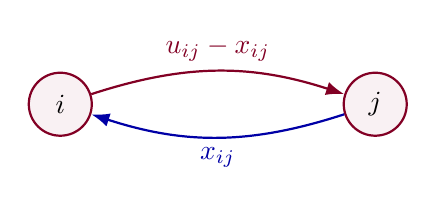
\begin{tikzpicture}[node/.style={circle,draw=sapienzared,thick,fill=softred,minimum size=8mm},arc/.style={-{Latex[length=2.3mm]},thick}]
\node[node] (i) at (0,0) {$i$}; \node[node] (j) at (4,0) {$j$};
\draw[arc,sapienzared] (i) to[bend left=18] node[above] {$u_{ij}-x_{ij}$} (j);
\draw[arc,blue!65!black] (j) to[bend left=18] node[below] {$x_{ij}$} (i);
\end{tikzpicture}
\caption{I due archi residui associati a un arco originale $(i,j)$.}
\end{figure}

\section{Cammini aumentanti}

\begin{definition}[Cammino aumentante]
Un cammino orientato da $s$ a $t$ nella rete residua è detto \emph{cammino aumentante}. La sua capacità residua è
\[
\Delta(P)=\min_{e\in P}r_e.
\]
\end{definition}

Lungo il cammino si aumenta di $\Delta(P)$ il flusso sugli archi originali percorsi direttamente e lo si diminuisce sugli archi originali percorsi inversamente. I bilanci ai nodi intermedi restano invariati e il valore del flusso cresce di $\Delta(P)>0$.

\begin{examplebox}{Perché servono gli archi inversi}
Una scelta iniziale può inviare flusso su un arco che in seguito si rivela poco conveniente. Un cammino residuo che usa l'arco inverso permette di ridurre quella decisione e reindirizzare il flusso. Cercare cammini soltanto sugli archi originali non è quindi corretto.
\end{examplebox}

\section{Ford-Fulkerson}

\begin{enumerate}
\item Partire da un flusso ammissibile, tipicamente $x=0$.
\item Costruire la rete residua $G_x$.
\item Se non esiste un cammino residuo da $s$ a $t$, terminare.
\item Scegliere un cammino aumentante $P$ e calcolare $\Delta(P)$.
\item Aggiornare il flusso lungo $P$ e tornare al passo 2.
\end{enumerate}

Se le capacità sono intere e il flusso iniziale è intero, ogni incremento è intero. Ne segue anche la proprietà di integralità: esiste un massimo flusso intero. Con capacità intere, Ford-Fulkerson termina dopo al più $f^*$ aumenti se ogni incremento è almeno uno; il limite è pseudo-polinomiale perché dipende dal valore delle capacità.

Con capacità irrazionali e una scelta sfavorevole dei cammini, il metodo generico può non terminare. Occorre pertanto specificare una regola di selezione.

\section{Edmonds-Karp}

L'algoritmo di Edmonds-Karp sceglie a ogni iterazione un cammino aumentante con il minor numero di archi, trovato mediante BFS nella rete residua.

\begin{theorem}[Complessità]
Edmonds-Karp termina in tempo
\[
O(|\V|\,|\E|^2),
\]
indipendentemente dai valori numerici delle capacità.
\end{theorem}

L'idea è che la distanza residua di ogni nodo dalla sorgente non diminuisce; inoltre, ogni arco può diventare critico solo un numero limitato di volte.

\begin{center}
\begin{tabular}{lll}
\toprule
Metodo & Scelta del cammino & Garanzia\\
\midrule
Ford-Fulkerson & arbitraria & finita con capacità intere\\
Edmonds-Karp & BFS, meno archi & $O(|\V||\E|^2)$\\
\bottomrule
\end{tabular}
\end{center}

\section{Teorema massimo flusso-minimo taglio}

\begin{theorem}[Max-flow min-cut]
Il valore del massimo flusso è uguale alla capacità del taglio $s$-$t$ minimo:
\[
\max\{f:x\text{ flusso ammissibile}\}
=
\min\{C(W,\Wbar):(W,\Wbar)\text{ taglio }s\text{-}t\}.
\]
\end{theorem}

\emph{Dimostrazione costruttiva.} Se non esiste un cammino aumentante, sia $W$ l'insieme dei nodi raggiungibili da $s$ nella rete residua. Allora $t\notin W$. Ogni arco originale da $W$ a $\Wbar$ è saturo, altrimenti sarebbe attraversabile residualmente; ogni arco da $\Wbar$ a $W$ è vuoto, altrimenti il suo inverso residuo renderebbe raggiungibile la coda. Pertanto
\[
f=F(W,\Wbar)=\sum_{e\in\delta^+(W)}u_e=C(W,\Wbar).
\]
Poiché ogni flusso è limitato superiormente da ogni taglio, flusso e taglio sono entrambi ottimi.

\begin{proposition}[Certificato di ottimalità]
Un flusso ammissibile è massimo se e solo se nella rete residua non esiste alcun cammino da $s$ a $t$.
\end{proposition}

Il flusso ottimo è un certificato primale; l'insieme dei nodi residualmente raggiungibili fornisce il certificato duale, cioè un taglio della stessa capacità.

\section{Esempio completo}

Consideriamo gli archi con capacità
\[
(s,a):4,quad (s,b):3,quad (a,b):2,quad (a,t):2,quad (b,t):5.
\]
Partendo dal flusso nullo:
\begin{enumerate}
\item sul cammino $s-a-t$ si inviano $2$ unità;
\item sul cammino $s-b-t$ si inviano $3$ unità;
\item sul cammino $s-a-b-t$ si inviano altre $2$ unità.
\end{enumerate}
Il valore finale è $f=7$. Nella rete residua, da $s$ non parte alcun arco con capacità positiva: il taglio $W=\{s\}$ ha capacità $4+3=7$. Flusso e taglio coincidono, dunque sono ottimi.

\section{Python e NetworkX}

\begin{networkxbox}
NetworkX usa l'attributo \texttt{capacity}. Le funzioni \texttt{maximum\_flow} e \texttt{minimum\_cut} restituiscono rispettivamente un flusso massimo e un taglio minimo. L'uguaglianza dei due valori è un controllo naturale del risultato.
\end{networkxbox}

\begin{lstlisting}[style=python,caption={Massimo flusso e taglio minimo con NetworkX}]
import networkx as nx

G = nx.DiGraph()
for i, j, u in [
    ("s", "a", 4), ("s", "b", 3),
    ("a", "b", 2), ("a", "t", 2),
    ("b", "t", 5)
]:
    G.add_edge(i, j, capacity=u)

value, flow = nx.maximum_flow(G, "s", "t")
cut_value, (W, Wbar) = nx.minimum_cut(G, "s", "t")

print("flusso massimo:", value)
print("taglio minimo:", cut_value, W, Wbar)
assert value == cut_value
\end{lstlisting}

È possibile selezionare l'algoritmo con il parametro \texttt{flow\_func}, per esempio usando la funzione \path{nx.algorithms.flow.edmonds_karp}. In presenza di numeri in virgola mobile è preferibile confrontare i valori con una tolleranza invece di usare l'uguaglianza esatta.

\section{Estensioni e trasformazioni}

\subsection{Più sorgenti o più pozzi}
Si introduce una supersorgente collegata alle sorgenti originarie e/o un superpozzo collegato ai pozzi originari. Le capacità dei nuovi archi rappresentano eventuali limiti di produzione o assorbimento; se tali limiti non esistono, si usa un valore superiore a ogni flusso possibile.

\subsection{Capacità sui nodi}
Un nodo $v$ con capacità $q_v$ viene sdoppiato in $v^{\mathrm{in}}$ e $v^{\mathrm{out}}$, collegati da un arco di capacità $q_v$. Gli archi entranti terminano nel primo nodo e quelli uscenti partono dal secondo.

\subsection{Archi non orientati}
Un collegamento non orientato può essere sostituito da due archi opposti. Occorre però chiarire se ciascuna direzione possiede capacità propria o se le due direzioni condividono un'unica capacità fisica.

\section{Registro delle notazioni}

\begin{notationbox}
\begin{center}
\begin{tabular}{ll}
\toprule
Simbolo & Significato\\
\midrule
$s,t$ & sorgente e pozzo\\
$x_{ij},u_{ij}$ & flusso e capacità sull'arco $(i,j)$\\
$f$ & valore del flusso\\
$(W,\Wbar)$ & taglio $s$-$t$\\
$\delta^+(W),\delta^-(W)$ & archi uscenti ed entranti nel taglio\\
$F(W,\Wbar)$ & flusso netto attraverso il taglio\\
$C(W,\Wbar)$ & capacità del taglio\\
$G_x$ & rete residua associata al flusso $x$\\
$r_e$ & capacità residua\\
$P,\Delta(P)$ & cammino aumentante e sua capacità\\
\bottomrule
\end{tabular}
\end{center}
\end{notationbox}

\section{Errori frequenti}
\begin{enumerate}
\item Imporre il bilancio nullo anche a $s$ e $t$ senza introdurre l'arco di ritorno.
\item Definire il valore del flusso usando soltanto gli archi uscenti da $s$ quando esistono archi entranti.
\item Sommare nel taglio minimo anche le capacità degli archi da $\Wbar$ a $W$.
\item Dimenticare gli archi inversi nella rete residua.
\item Aumentare il flusso su un arco percorso inversamente invece di diminuirlo.
\item Fermarsi perché non si trova un cammino nel grafo originale, anziché nella rete residua.
\item Considerare il valore massimo senza fornire un taglio che ne certifichi l'ottimalità.
\end{enumerate}

\section{Esercizi}

\textbf{Esercizio 6.1 -- Ammissibilità.}
Dato un vettore di flusso su una rete $s$-$t$, verificare capacità, bilanci e valore $f$.

\medskip\textbf{Esercizio 6.2 -- Tagli.}
Enumerare tutti i tagli $s$-$t$ di una rete con cinque nodi, calcolarne le capacità e individuare un limite superiore al massimo flusso.

\medskip\textbf{Esercizio 6.3 -- Rete residua.}
Costruire la rete residua di un flusso assegnato, includendo tutti gli archi inversi di capacità positiva.

\medskip\textbf{Esercizio 6.4 -- Ford-Fulkerson.}
Applicare l'algoritmo partendo dal flusso nullo, indicando a ogni iterazione cammino, incremento e flusso aggiornato.

\medskip\textbf{Esercizio 6.5 -- Certificato.}
Al termine dell'Esercizio 6.4 determinare i nodi raggiungibili da $s$ nella rete residua e verificare l'uguaglianza flusso-taglio.

\medskip\textbf{Esercizio 6.6 -- NetworkX.}
Implementare l'esempio del capitolo, confrontare \texttt{maximum\_flow} e \texttt{minimum\_cut}, quindi ridurre una capacità e analizzare il nuovo taglio minimo.

\section{Sintesi del capitolo}
\begin{learningbox}
\begin{itemize}[nosep]
\item Il massimo flusso è un caso particolare del flusso a costo minimo.
\item Ogni taglio $s$-$t$ fornisce un limite superiore al valore del flusso.
\item La rete residua rappresenta aumenti e possibili annullamenti del flusso corrente.
\item Ford-Fulkerson aumenta il flusso finché esiste un cammino residuo $s$-$t$.
\item Edmonds-Karp usa cammini BFS e ha complessità polinomiale.
\item Un flusso è massimo se e solo se coincide con la capacità di un taglio minimo.
\end{itemize}
\end{learningbox}

\paragraph{Verso il capitolo successivo.}
Il prossimo problema fondamentale sarà quello dei cammini minimi. Anche in quel caso partiremo dal flusso a costo minimo e ritroveremo potenziali e costi ridotti con una nuova interpretazione.

\end{document}
